\documentclass[12pt]{report}

\usepackage{amsmath}
\usepackage{pgfplots}
\usepgfplotslibrary{units}
\usepackage[russian]{babel}
\usepackage{filecontents}
\usepackage{titlesec, blindtext, color}
\usepackage{listings}
\usepackage{pdfpages}

\usepackage{titlesec, blindtext, color} 
\definecolor{gray75}{gray}{0.75} 
\newcommand{\hsp}{\hspace{20pt}} 

\setcounter{tocdepth}{3}
\setcounter{secnumdepth}{3}

\usepackage{geometry}
\geometry{top=0.5cm}

\lstset{
	language=C++,
	numbers=left,
	breaklines=true, 
	frame=single,
	texcl=true,
	basicstyle=\ttfamily,
	extendedchars=\true
}

\titleformat{\chapter}[hang]{\Huge\bfseries}{\thechapter\hsp\textcolor{gray75}{|}\hsp}{0pt}{\Huge\bfseries}

\begin{filecontents}{ZG1.dat}
	160000 0.21
	320000 0.261 
	560000 0.306
	880000 0.411
	1280000 0.573
	2480000 1.526 
	3280000 2.688
\end{filecontents}

\begin{filecontents}{ZPH1.dat}
	160000 0.51
	320000 0.555
	560000 0.718
	880000 0.904
	1280000 1.128
	2480000 2.149 
	3280000 2.934
\end{filecontents}

\begin{filecontents}{RT1.dat}
	160000 1.261
	320000 1.271
	560000 1.356
	880000 1.514
	1280000 1.684
	2480000 1.972
	3280000 2.073
\end{filecontents}

\begin{filecontents}{RT2.dat}
	24 1.675
	48 3.095
	60 3.793
	72 4.609
	84 5.155
\end{filecontents}

\begin{filecontents}{ZPH2.dat}
	24 0.245
	48 0.485
	60 0.593
	72 0.702
	84 0.751
\end{filecontents}

\begin{filecontents}{ZG2.dat}
	24 0.348
	48 0.242
	60 0.247
	72 0.25
	84 0.259
\end{filecontents}



\begin{document}

	a
	\newpage
	b
	\newpage
	\tableofcontents
	\chapter*{Введение}
	\addcontentsline{toc}{chapter}{Введение}
	В наше время одна из основных задач компьютерной графики состоит в создании и развитии алгоритмов построения реалистичных изображений. Данные алгоритмы используются повсеместно, например: компьютерные игры, дизайн, кинематограф и т.д. 
	
	Для построения изображения, максимально похожего на то, что мы видим в реальной жизни, необходимо учитывать такие явления как: преломление, отражение, рассеивание света и многие другие.
	
	На данный момент существует множество алгоритмов для синтеза реалистичного изображения, каждый из которых имеет свои достоинства и недостатки. 
	
	\textbf{Цель данной работы} - реализовать и сравнить алгоритм Z-буфера с закраской по Гуро, алгоритм Z-буфера с закраской по Фонгу и алгоритм обратной трассировки лучей.
	
	Для достижения поставленной задачи необходимо:
	\begin{enumerate}
		\item проанализировать рассматриваемы алгоритмы компьютерной графики;
		\item реализовать данные алгоритмы;
		\item провести сравнительный анализ.
	\end{enumerate}

	Итогом работы над данным проектом должны стать программа, демострирующая работу этих алгоритмов, а также выводы, сделанные на основе проведенного сравнительного анализа.
	
	\chapter{Аналитическая часть}
	\section{Формализация сцены}
	
		На сцене могут располагаться некоторые колличество геометрических объектов: икосаэдров, параллелипипедов и прямых трехгранных призм. Положение и размер икосаэдра должен задаваться координатами центра описанной окружности и её радиусом, параллелипипеда - также координатами центра, шириной, высотой и глубиной, прямой трехгранной призмы - так же как и параллелипипеда.
		
		Каждый объект обладает характеристиками: цвет, коэффициент рассеивания, коэффициент отражения, коэффициент блеска.
		
		На сцене также могут находиться некоторые количество точечных источников света. Каждый источник задается координатой в пространстве и интенсивность.
		
	\section{Представление объектов сцены}
	
	Необходимо выбрать модель представления объектов на сцене. Для реализации поставленной задачи предпочтительнее будет использовать поверхностные модели, так как для синтеза реалистичного изображения необходимо знать только внешний вид изображаемого объекта.
	
	Для задания поверхностной модели я буду использовать полигональную сетку. Полигональная сетка – представление поверхности геометрического объекта в виде набора состыкованных друг с другом плоских полигонов. В качестве полигонов мою были выбраны треугольники, так как это, в дальнейшем, упростит производимые расчеты.
	
	Существует множество представлений полигональной сетки. Ниже я рассмотрю четыре, по моему мнению, основных представления: Вершинное, Список граней, «Крылатое» и Веер треугольников.
	
	\begin{itemize}
		\item Вершинное представление – описывает объект как множество вершин, соединенных с другими вершинами. Дает выигрыш по памяти, но проигрыш в скорости обхода.
		\item Список граней – представляет объект как множество граней и множество вершин. Требует больше памяти, чем вершинное представление, но позволяет находить соседние грани и вершины за постоянное время.
		\item «Крылатое» представление – явно представляет вершины, грани и ребра сетки. Требует значительно больше памяти чем список граней и вершинное представление, но позволяет увеличить скорость обхода сетки.
		\item Веер треугольников – описывает множество соединенных треугольников, которые делят одну центральную вершину. Данное представление требует мало памяти и позволяет производить быстрый обход сетки, но требует больших затрат при изменении.
	\end{itemize}

	В данной работе мною будет использован список граней, так как я считаю, что в данной работе допустимо пренебречь дополнительными затратами по памяти ради уменьшения затрат на написания программного продукта.

	\section{Анализ рассматриваемых алгоритмов}
	
	\subsection{Алгоритм, использующий Z-буфер}
	
	Идея алгоритма, использующего Z-буфер, заключается в наличии двух буферов: буфер кадра и буфер глубины (он же Z-буфер). В первом хранится информация об атрибутах каждого пикселя экрана. Второй используется для хранения Z координаты каждого пикселя. 
	
	Перед началом работы данного алгоритма, каждый, находящийся на сцене объект, переводится в растр. Далее необходимо пройти по всем пикселям каждого объекта. В процессе прохода координата Z каждого нового пикселя сравнивается со значением, записанным в Z-буфере. Если сравнение показывает, что Z координата нового пикселя больше записанного, то новый пиксель заносится в буфер кадра. Также производится запись новой координаты Z в соответствующее значение Z-буфера. В ином случае никаких действий не производится.
	
	Основное преимущество этого алгоритма заключается в его простоте. Также он позволяет обрабатывать объекты в произвольном порядке, что позволяет экономить время, затрачиваемое на сортировку по глубине.
	
	Основной недостаток алгоритма – большой объем требуемой памяти. Другой недостаток заключается в трудоемкости реализации эффектов прозрачности и просвечивания.

	\subsection{Метод Гуро}

	Метод Гуро – метод закрашивания в трехмерной компьютерной графики (так же еще называют методом затемнения и сглаживания). 
	Данный метод основывается на идеи закрашивания каждого полигона не одним цветом, а плавно изменяющимися оттенками, вычисляемыми путем интерполяции цветов примыкающих граней. Так как в нашем случае каждая грань является треугольником, достаточно вычеслить освещенность в каждой вершине и далее путем билинейной интерполяции находить освещенность в каждой точке грани. 
	
	К недостаткам метода Гуро относят то, что он хорошо работает только с диффузной моделью отражения. 

	\subsection{Метод Фонга}
	Метод Фонга – также является методом закрашивания (затемнения, сглаживания), основой которого является интерполяция векторов нормалей. В нашем случае объект представляет собой множество плоских граней, соответственно для реализации метода Фонга достаточно найти нормаль в каждой грани, и на её основе вычислять освещенность для каждого пикселя.
	
	Этот метод требует больших вычислительных затрат, чем метод Гуро, но дает в итоге позволяет получить более качественное изображение, так как в данном методе освещенность вычислется для пикселя грани, а не только для её вершин, как в метода Гуро.
	
	\subsection{Растровая развертка треугольника}
	
	Для разложения треугольница в растр изначально производится одновременное разложение в растр двух ребер рассматриваемого треугольника методом цифрового дифференциального анализатора (ЦДА). При вычислении новых значений точек, принадлежащих кадому из отрезков, производится разложение в растр отрезка, полученного из двух найденных точек. Таким образом получается найти все точки принадлежащие рассматриваемому треугольнику.
	
	На данном рисунке точки $a$, $b$, $c$ это точки образующие треугольник. Точка $ab'$ - это точка принадлежащая отрезку $ab$, полученная в результате перевода в раст этого отрезка. Точка $ac'$ - точка, соответственно, принадлежащая отрезку $ac$. Стрелочками показано направление движение при переводе в растр.
	\begin{center}
		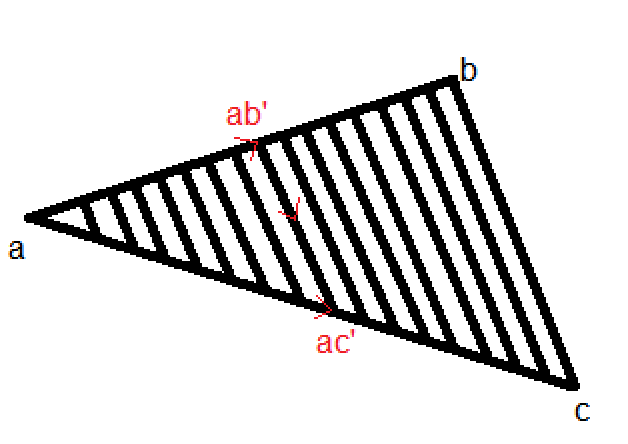
\includegraphics[scale=0.7]{cda.png}
		
		Рис. 1.1. Пример разложения треугольника в растр.
	\end{center}
	
	\subsection{Обратная трассировка лучей}
	Идея обратной трассировки лучей заключается в том, что из виртуального глаза, находящегося на некотором расстоянии от экрана, испускается луч и находится точка его пересечения с объектом сцены. Далее определяется освещенность найденной точки. Делается это путем испускания из данной точки лучей ко всем источникам света и определения их вклада в общую освещенность. Далее из найденной точки пересечения рекурсивно испукается отраженный луч, для поиска объектов, отражающихся в данном. Данный процесс повторяется до тех пор, пока луч не выходит за пределы сцены. Также этот процесс можно ограничить максимальной глубиной рекурсии. 
	
	Данный алгоритм позволяет не только закрашивать объекты, но также и определять их видимость, что делает его достаточно универсальным.
	Достоинства обратной трассировки лучей:
	\begin{itemize}
		\item возможность рендеринга гладких объектов без их предварительной аппроксимации;
		\item возможность эффективного распараллеливания вычислений.
	\end{itemize}

	Основным недостатком этого алгоритма является относительно низкая производительность.
	
	\section*{Вывод}
	\addcontentsline{toc}{section}{Вывод}
	
	В данном разделе был осуществлен выбор способа хранения информации об объектах. Выбор пал на список граней, так как он позволяет уменьшить затраты на написание программного продукта из-за простоты своей реализации. На ряду с этим были описанны рассматриваемые алгоритмы.
	
	\chapter{Конструкторская часть}
	\section{Модель освещения Фонга}
	
	В данной работе было решено использовать модель освещения Фонга. Данная модель учитывает три компоненты освещения: Фоновую (ambient), рассеянную (diffuse) и зеркальную (specular).
		
	Фоновое освещение присутствует в любом уголке сцены. Это происходит из-за многократного отражения лучей света от окружающих объектов. 
		
	Рассеянное освещение – тот свет, что отражается от поверхности во всех направлениях.
	
	Зеркальное освещение – часть отраженных лучей, попадающих в глаза наблюдателю.
	
	Для вычисления общей освещенности от одного точечного источки в некоторой точке пространства будет использована формула:
	\begin{equation}
		I = I_{a} + K_{d}*(\overline{n}, \overline{l})*I_{n} + K_{s}*(\overline{V}, \overline{R})^{p}*I_{n}
	\end{equation}
		
		$I_{a}$ - интенсивность фонового освещения
		
		$K_{d}$ - коэффициент рассеянного освещения
		
		$K_{s}$ - коэффициент зеркального освещения
		
		$P$ - коэффициент блеска
		
		$I_{n}$ - мощность n-го источника света, расчитывается как
		
		$\overline{n}, \overline{l}, \overline{V}, \overline{R}$ - единичные вектора. Нормаль, до источника света, до точки наблюдения, отраженного луча. 
		~\\
		
		Если источников больше одного, тогда для вычисления итоговой освещенности необходимо сложить вклад в рассеянное и зеркальное отражение каждого источника.
		
	\section{Метод Гуро}
	
	Описание алгоритма:
	
	\begin{enumerate}
		\item расчитать нормаль к каждой грани (так как в данном случае каждая грань является треугольником, нормаль можно вычислить путем векторного произведения двух сторон);
		\item определить нормаль в вершинах рассматриваемой грани, путем усреднения нормалей примыкающих граней;	
		\item закрасить грань цветом, соответствующим билинейной интерполяции значений интенсивности в вершинах.
	\end{enumerate}

	Рассмотрим билинейную интерполяцию интенсивностей.
	
	\begin{center}
		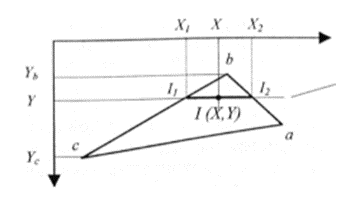
\includegraphics[scale=1]{gourand.png}
		
		Рис. 2.1. Пример билинейной интерполяции интенсивностей.
	\end{center}

	Интенсивность $I$ определяется исходя из пропорции:
	\begin{equation}
		(I - I_{1})/(X - X_{1}) = (I_{2} - I_{1})/(X_{2} - X_{1})
	\end{equation}
	Отсюда следует:
	\begin{equation}
		I = I_{1} + (I_{2} - I_{1})(X - X_{1})/(X_{2} - X_{1})
	\end{equation}
	
	Значения $I_{1}$, $I_{2}$ расчитываются как:
	\begin{equation}
		I_{1} = I_{b} + (I_{c} - I_{b})(Y - Y_{b})/(Y_{c} - Y_{b})
	\end{equation}
	\begin{equation}
		I_{2} = I_{b} + (I_{a} - I_{b})(Y - Y_{b})/(Y_{a} - Y_{b})
	\end{equation}
	
	\section{Метод Фонга}
	
	Описание алгоритма:
	\begin{enumerate}
		\item вычисление нормали к рассматриваемой грани;
		\item произвести расчет освещенности каждого пикселя грани, на основе вычисленной нормали.
	\end{enumerate}

	\section{Алгоритм, использующий Z-буфер}
	
	Описание алгоритма:
	\begin{enumerate}
		\item элементам буфера кадра присвоить значение цвета фона;
		\item элементам Z-буфера присвоить минимальное значение типа данных;
		\item для каждого треугольника, кажого объекта на сцене:
		\begin{enumerate}
			\item выполнить растровую развертку треугольника;
			\item для каждого пикселя, принадлежащего грани, сравнить координату Z с соответствующим значением, хранящемся в Z-буфере:
			\begin{enumerate}
				\item если больше: 
				\begin{enumerate}
					\item в буфер кадра записать атрибуты рассматриваемого пикселя (по соответствующим X, Y);
					\item записать значение координаты Z рассматриваемого пикселя в Z-буфер (по соответствующим X, Y);
				\end{enumerate}	
			\end{enumerate}
		\end{enumerate}
		\item отобразить полученное изображение.
	\end{enumerate}

	\section{Растровая развертка треугольника}
	
	Пусть треугольник задается тремя точками $A$, $B$, $C$.
	
	Описание алгоритма:
	\begin{enumerate}
		\item найти единичный вектор движения вдоль отрезка $AB$, как $|\overline{AB}|$;
		\item найти единичный вектор движения вдоль отрезка $AC$, как $|\overline{AC}|$;
		\item инициализировать начальную точку для движения вдоль $AB$, $T1 = A$;
		\item инициализировать начальную точку для движения вдоль $AC$, $T2 = A$;
		\item пока точка $T1 != B$ и $T2 != C$
		\begin{enumerate}
			\item перевести в растр отрезок $T1T2$;
			\item сместить $T1$ на $|\overline{AB}|$, $T2$ на $|\overline{AC}|$;
		\end{enumerate}
		\item отобразить полученное изображение.
	\end{enumerate}

	\section{Обратная трассировка лучей}

	Описание алгоритма:
	\begin{enumerate}
		\item для каждого пикселя экрана:
		\begin{enumerate}
			\item задать направление пускаемого луча, $|\overline{VP}|$, $V$ - точка наблюдателя, $P$ - текущая точка экрана
			\item для каждого объекта сцены:
			\begin{enumerate}
				\item найти пересечения со сферой, описанной вокруг объекта;
				\item если пересечение есть, найти точку пересечения с каждой гранью этого объекта:
				\item если точка есть:
				\begin{enumerate}
					\item расчитать освещенность найденной точки;
					\item если не достигнута максимальная глубина рекурсии, рекурсивно пустить отраженный луч и прибавить найденное значение к текущему цвету пикселя;
				\end{enumerate}
				\item иначе установить цвет пикселя равному цвету фона;
			\end{enumerate}
			\item закрасить текущую точку экрана соотвествуя найденному значению;
		\end{enumerate}
	\end{enumerate}	

	\section{Поиск пересечения луча со сферой}
	
	Луч задается уравнением:
	\begin{equation}
		\overline{r} = \overline{o} + t*\overline{d}
	\end{equation}
	
	$t \in R, t >= 0$
	
	$\overline{o}$ - начальная точка луча
	
	$\overline{d}$ - направление луча
	
	Координаты этого луча можно записать как:
	\begin{equation}
		X = X_{o} + t*X_{d}
	\end{equation}
	
	\begin{equation}
		Y = Y_{o} + t*Y_{d}
	\end{equation}
	
	\begin{equation}
		Z = Z_{o} + t*Z_{d}
	\end{equation}
	
	
	Сфера задается уравнением:
		
	\begin{equation}
		(X - X_{c})^2 + (Y - Y_{c})^2 + (Z - Z_{c})^2 = R^2
	\end{equation}
	
	Для того, чтобы найти пересечение луча со сферой необходимо в уравнение сферы подставить соотвествующие координаты луча.
	
	После подстановки и несложных преобразований можно получить:
	\begin{equation}
		t^2 + B*t + C = 0
	\end{equation}
	
	Где,
	\begin{equation}
		B = 2(X_{d}*(X_{o} - X_{c}) + Y_{d}*(Y_{o} - Y_{c}) + Z_{d}*(Z_{o} - Z_{c}))
	\end{equation}
	
	\begin{equation}
		C = (X_{o} - X_{c})^2 + (Y_{o} - Y_{c})^2 + (Z_{o} - Z_{c})^2 - R^2
	\end{equation}
	
	Если дискриминант этого уравнения меньше нуля, тогда луч не пересекается со сферой. Иначе найденные корни будут являться параметрами, которые необходимо подставить в уравнение (2.6) для того, чтобы найти необходимые точки пересечения.
	
	При написании данной работы поиск пересечения со сферой необходим для оптимизации работы обратной трассировки лучей. В этом случае нас интерисует только факт того, есть пересечение или нет, соответственно достатоно лишь проверить знак дескрименанта.
	
	\section{Поиск пересечения луча с треугольником}
	
	Пусть луч задается так же, как и при поиске пересечения со сферой (2.6).
	
	Тогда для поиска пересечения с треугольником, изначально необходимо найти точку пересечения этого луча с плоскостью, образованной этим треугольником.
	
	Точка $\overline{p}$ лежит в плоскости, если $(\overline{p} - \overline{q})*\overline{n} = 0$. 
	
	$\overline{n}$ - нормаль к плоскости.
	
	Если подставить вместо $\overline{r}$ координаты луча и выразить параметр, то можно получить:
	\begin{equation}
		t = \frac{(\overline{q} - \overline{o})*\overline{n}}{\overline{d}*\overline{n}}
	\end{equation}
	
	Если $t$ < 0, то точки пересечения нет, иначе $\overline{r} = \overline{o} + t*\overline{d}$ искомая точка пересечения.
	
	Далее необходимо определить, принадлежит ли найденная точка, если таковая имеется, треугольнику.
	
	Пусть треугольник задается тремя точками $A$, $B$, $C$, а найденную точку назовем $P$.
	
	Тогда, если результат трех векторных произведений $\overline{AB}$x$\overline{AP}$, $\overline{BC}$x$\overline{BP}$ и $\overline{CA}x\overline{CD}$ будут сонаправлены, то точка $P$ лежит внутри треугольника $ABC$. Сонаправленность можно проверить путем сравнения знака соответсвующих координат полученных векторов.
	
	\section{Поиск отраженного луча}

	Отраженный луч ищется как:
	\begin{equation}
		\overline{r} = \overline{d} - 2\overline{n}*(\overline{d}*\overline{n})
	\end{equation}
	
	$\overline{d}$ - направление падающего луча
	
	$\overline{n}$ - нормаль в точке падения

	\section{Оценка трудоемкости алгоритмов}
	
	\subsection{Оценка трудоемкости Z-буфрера с закраской по Гуро}
	
	Трудоемкость Z-буфера с использованием закраски по методу Гуро состоит из трудоемкости перевод каждой грани в растр, подсчета освещенности вершин и последующей их интерполяции.
	
	Из этих трех операций, самой затратной является подсчет освещенности в вершинах, поэтому далее будет оцениваться трудоемкость всего алгоритма именно по этой операции.
	
	В данном алгоритме подсчет освещенности происходит трижды для каждой грани, из чего следует, что трудоемкость данного алгоритма линейно зависит от колличества граней с маленькой константой равной 3.
	
	\subsection{Оценка трудоемкости Z-буфреа с закраской по Фонгу}
	
	Также как и в предыдущем пункте, трудоемкость алгоритма будет расчитываться по колличеству расчетов освещенности в точке.
	
	Так как в метода закраски по Фонгу освещенность требуется рассчитывать для каждой точки грани, то трудоемкость линейно зависит от суммарной площадли всех граней каждого объекта на сцене.
	
	\subsection{Оценка трудоемкости обратной трассировки лучей}

	В данном алгоритме наибольших затрат требует поиск пересечение луча с объектом.
	
	Так как для поиска пересечения с объектом требуется найти точку пересечения с каждой гранью, то из этого можно сделать вывод, что трудоемкость обратной трассировки лучей линейно зависит от сумарного колличества граней объектов, но с очень большой константой, равной разрешению экрана, на которой идет проецирование изображения.

	\section*{Вывод}
	\addcontentsline{toc}{section}{Вывод}

	В данном разделе были описаны принципы работы всех рассматриваемых алгоритмов, а также необходимые для расчетов математические соотношения.
	
	\chapter{Технологическая часть}
	
	\section{Выбор языка и среды программирования}
	
		Для реализации данного программного продукта был выбран язык C++, так как имеется наибольший опыт работы с данным языком.
		
		Также была выбрана объектно-ориентированная технология из-за её гибкости и из-за того что она предоставляет возможность вносить правки в уже написанный код без необходимости переписывания больших его частей.
		
		Для реализации интерфейса был выбран фреймворк QT, так как он предоставляет большой спектр возможностей для создания сложных интерфейсов.
		
		C++ предоставляет доступ к библиотекам для параллельного программирования. В данной работе будут использованы <thread> для создания параллельных потоков и <mutex> для ограничения доступа к ресурсам.
		
	\section{Замеры времени}
	Замер времени работы алгоритмов производился при помощи функций clock() из библиотеки time.h.
	
	\newpage
	\section{Интерфейс программы}
	
	На Рис. 3.1. представлен пользовательский интерфейс программы. Слева - инструментарий для редактирования сцены, справа синтезированное изображение.
	
	\begin{center}
		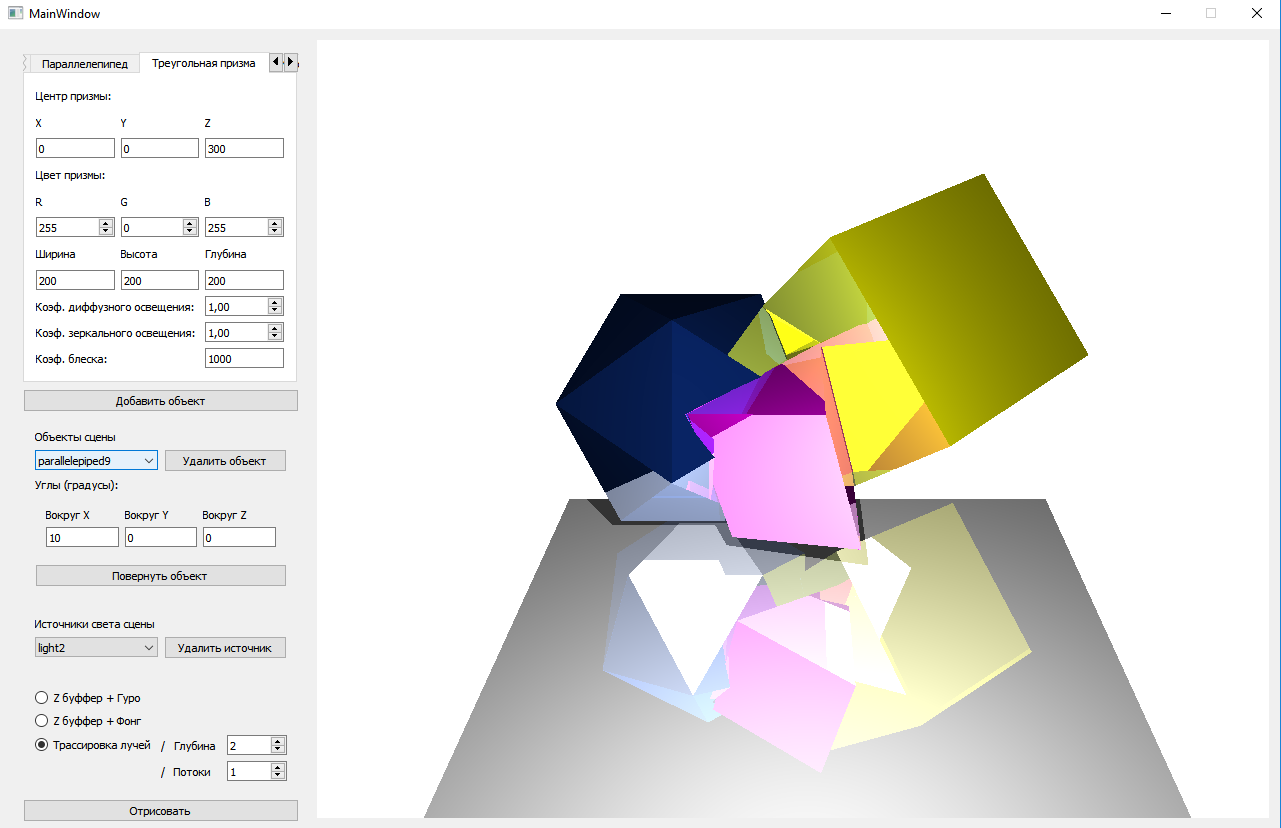
\includegraphics[scale=0.45]{UI.png}
		
		Рис. 3.1. Интерфейс программы
	\end{center}	

	
	На Рис. 3.2. - Рис. 3.4. изображены окна добавления объектов на сцену.
	Каждое окно имеет поля для ввода:
	\begin{enumerate}
		\item центра фигуры;
		\item цвета фигуры;
		\item коэффициента диффузного и зеркально освещения;
		\item коэффициент блеска;
		\item параметры, необходымые для задания размеров объекта (Радиус для икосаэдра, Ширина, Высота и Глубина для параллелепипеда и прямой треугольной призмы)
	\end{enumerate}

	На Рис. 3.5. изображено окно добавления источника света. Данное окно обладает полями для ввода координаты источника и его интенсивности.
	
	Переключение между окнами происходит при помощи стрелок, расположенных в правом верхнем углу.
	
	~\\
	
	\begin{minipage}{0.5\textwidth}
		%\flushleft
			\begin{center}
				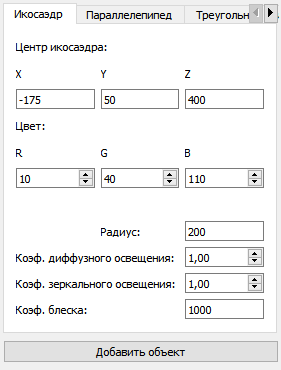
\includegraphics[scale=0.8]{ico.png}
				
				Рис. 3.2. Окно добавление икосаэдра
			\end{center}
	\end{minipage}
	\hfill
	\begin{minipage}{0.5\textwidth}
		\begin{center}
			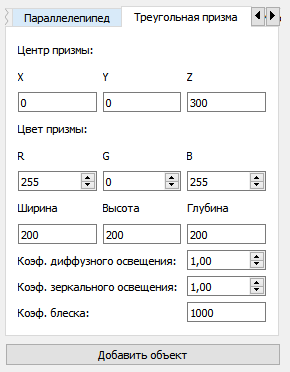
\includegraphics[scale=0.8]{prism.png}
			
			Рис. 3.4. Окно добавление трехгранной прямой призмы
		\end{center}
	\end{minipage}

		\begin{minipage}{0.5\textwidth}
		%\flushleft
		\begin{center}
			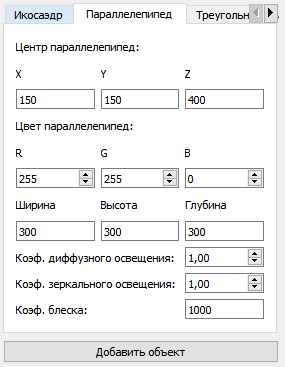
\includegraphics[scale=0.8]{paral.png}
			
			Рис. 3.3. Окно добавление параллелепипеда
		\end{center}
	\end{minipage}
	\hfill
	\begin{minipage}{0.5\textwidth}
		\begin{center}
			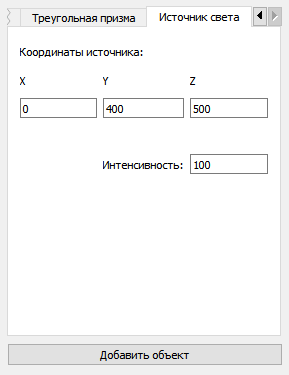
\includegraphics[scale=0.8]{lt.png}
			
			Рис. 3.5. Окно добавление источника света
		\end{center}
	\end{minipage}

	На Рис. 3.6. изображены поля, предоставляющие доступ для изменения и удаления объектов, уже находящихся на сцене.
	
	Все созданные объекты добавляются в список, далее можно выбрать объект из этого списка и удалить или повращать его.
	
	Источники света добавляются в отдельный список, их можно только удалять.

	\begin{center}
		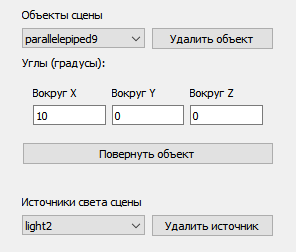
\includegraphics[scale=1]{changes.png}
		
		Рис. 3.6. Поля для изменения созданных объектов
	\end{center}
	
	На Рис. 3.7 изображены поля для выбора способа синтеза изображения.
	
	Поле Глубина отвечает за максимальную глубину рекурсии при поиске отраженных лучшей для алгоритма обратной трассировки лучей.
	
	Поле Потоки отвечает за то, на сколько потоков будет делиться процесс при синтезе изображения.
	
	\begin{center}
		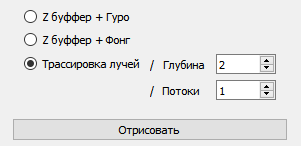
\includegraphics[scale=1]{choose.png}
		
		Рис. 3.7. Поля для выбора способо синтеза изображения
	\end{center}

	\section*{Вывод}
	\addcontentsline{toc}{section}{Вывод}
	
	В данном разделе был обоснован выбор языка программирования, описаны выбранные средства для создания интерфейка, а так как же описано строение пользовательского интерфейка.


	\chapter{Экспериментальная часть}
	
	\section{Цель эксперимента}
	
	Целью эксперимента является временное и качественное сравнение работы реализованных алгоритмов.
	
	\section{Апробация}
	
	На Рис. 4.1. представлена сцена, содержащая куб, икосаэдр, трехгранную призму и один точечный источник. Это изображение сгенерировано обратной трассировкой лучей.
	
	\begin{center}
		\includegraphics[scale=0.8]{rt.png}
		
		Рис. 4.1. Сцена, сгенерированая обратной трассировкой лучей.
	\end{center}

	Таже самая сцена, так же сгенерированная обратной трассировкой, но в данном случае вычислялись отражения.
	
	\begin{center}
		\includegraphics[scale=0.8]{rto.png}
		
		Рис. 4.2. Сцена, сгенерированая обратной трассировкой лучей и отражениями.
	\end{center}

	Сцена, сгенерированная с использованием Z-буфера и метода Фонга.

	\begin{center}
		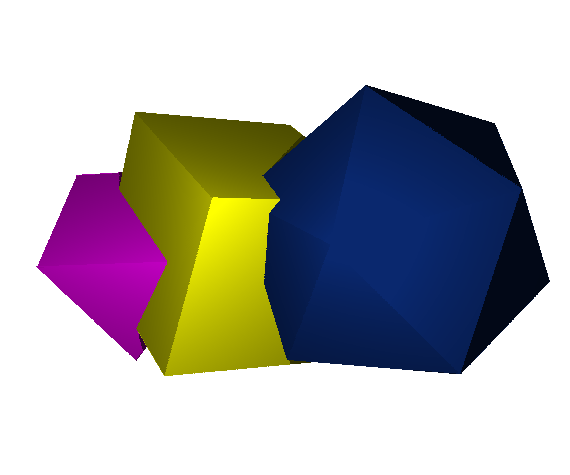
\includegraphics[scale=0.8]{gph.png}
		
		Рис. 4.3. Сцена, сгенерированая Z-буфером и методом Фонга.
	\end{center}

	Сцена, сгенерированная с использованием Z-буфера и метода Гуро.

	\begin{center}
		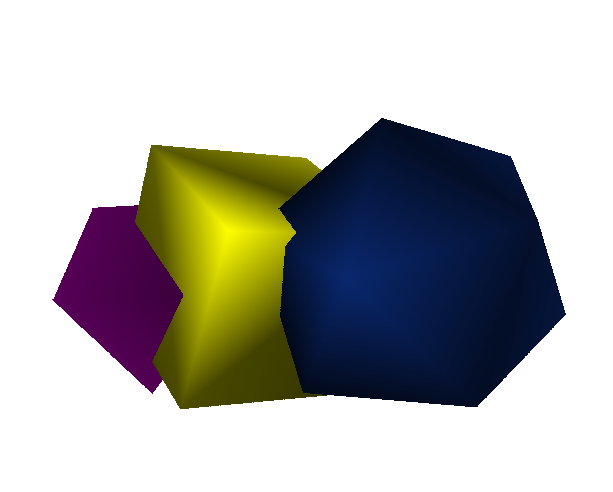
\includegraphics[scale=0.8]{zg.png}
		
		Рис. 4.4. Сцена, сгенерированая Z-буфером и методом Гуро.
	\end{center}

	\section{Описание эксперимента}
	
	Суть эксперимента заключается в том, чтобы замерить скорость работы алгоритмов в 
	двух различных случаях.
	
	Первый случай - когда суммарное колличество граней объектов на сцене не изменяется, увеличивается лишь суммарная площадь этих граней. В теории этот случай должен быть благоприятен для использования трассировки лучей.
	
	Второй - обратная, когда увеличивается суммарное колличество граней при неизменной площади. В теории этот случай должен быть благоприятен для использования Z-буфера с Фонгом или же с Гуро.
	
	Эксперимент проводоился на компьютере с:
	\begin{enumerate}
		\item Intel(R) Core(TM) i7-3770K
		\item 8.00 ГБ ОЗУ
	\end{enumerate}

	\subsection{Первый случай}
	
	В данном случае был создан один объект - парраллелипипед, содержащий 12 треугольников - граней.
	Во время эксперимента увеличивались длины ребер, тем самым увеличивая площадь объекта.
	
	Новых объектов не добавлялось, соответственно суммарное колличество граней не изменялось.
	
	Таблица. 4.1. Сравнение алгоритмов при увелечении площади граней.
	
	\begin{center}
		\begin{tabular}{|c c c c|}
			\hline
			Площадь (px) & Z+gourand (c) & Z+phong (c) & RayTrace (c) \\ [0.5ex]
			\hline
			160000 & 0.21 & 0.51 & 1.261 \\ 
			\hline 
			320000 & 0.261 & 0.555 & 1.271 \\ 
			\hline 
			560000 & 0.306 & 0.718 & 1.356 \\ 
			\hline 
			880000 & 0.411 & 0.904 & 1.514 \\ 
			\hline 
			1280000 & 0.573 & 1.128 & 1.684 \\ 
			\hline 
			2480000 & 1.526 & 2.149 & 1.972 \\ 
			\hline 
			3280000 & 2.688 & 2.934 & 2.073 \\
			\hline
		\end{tabular}
	\end{center}

	\begin{center}
		\begin{center}
			\begin{tikzpicture}
			\begin{axis}[
			axis lines = left,
			xlabel = $\texttt{Площадь (px)}$,
			ylabel = $\texttt{Время (сек.)}$,
			legend pos=outer north east,
			ymajorgrids=true
			]
			
			\addplot[color=green] table[x index=0, y index=1] {RT1.dat};
			\addplot[color=blue] table[x index=0, y index=1] {ZPH1.dat};
			\addplot[color=red] table[x index=0, y index=1] {ZG1.dat};
			
			\addlegendentry{RayTrace}
			\addlegendentry{Z-buff + Phong}
			\addlegendentry{Z-buff + gourand}
			\end{axis}
			\end{tikzpicture}
		\end{center}
		Рис. 4.5. График сравнения алгоритмов при увеличении площади граней.
	\end{center}

	Видно, как при сильном увеличении суммарной площади без увеличения колличества граней на сцене, в трассировка лучей начинает выигрывать у Z-буфера с Гуро и Z-буфера с Фонгом. (Таблица )
	
	Это связано с тем, что алгоритм Z-буфера переводит в растр все грани каждого объекта, соотвественно при увеличении площади увеливается и трудоемкость.
	
	В тоже время обратная трассировка лучей лишь находит точку пересечения с гранью и никак не зависит от её площади.
	
	Из этого эксперимента можно сделать вывод, что обратную трассировку лучей выгоднее использовать для синтеза сцены, на которой малое колличество граней, но их суммарная площадь велика.
	
	Видно, что трассировка начала работать быстрее только суммарной площади равной 3280000. При таком значении трассировка быстрее алгоритмов с Z-буфером приверно в 1.45 раз.
	
	\subsection{Второй случай}
	
	Во втором случае был проведет обратный первому эксперимент. 
	
	Площадь была зафиксированна в значении 60000 px. На этот раз добавлялись новые объекты, тем самым увеличивая суммарное колличество ребер.
	\newpage
		Таблица. 4.1. Сравнение алгоритмов при увелечении площади граней.
	
	\begin{center}
		\begin{tabular}{|c c c c|}
			\hline
			Кол-во ребер & Z+gourand (c) & Z+phong (c) & RayTrace (c) \\ [0.5ex]
			\hline
			24 & 0.348 & 0.245 & 1.675 \\ 
			\hline 
			48 & 0.242 & 0.485 & 3.095 \\ 
			\hline 
			60 & 0.247 & 0.593 & 3.793 \\ 
			\hline 
			72 & 0.25 & 0.702 & 4.609 \\ 
			\hline 
			84 & 0.259 & 0.751 & 5.155 \\ 
			\hline
		\end{tabular}
	\end{center}

	\begin{center}
		\begin{center}
			\begin{tikzpicture}
			\begin{axis}[
			axis lines = left,
			xlabel = $\texttt{Кол-во ребер}$,
			ylabel = $\texttt{Время (сек.)}$,
			legend pos=outer north east,
			ymajorgrids=true
			]
			
			\addplot[color=green] table[x index=0, y index=1] {RT2.dat};
			\addplot[color=blue] table[x index=0, y index=1] {ZPH2.dat};
			\addplot[color=red] table[x index=0, y index=1] {ZG2.dat};
			
			\addlegendentry{RayTrace}
			\addlegendentry{Z-buff + Phong}
			\addlegendentry{Z-buff + gourand}
			\end{axis}
			\end{tikzpicture}
		\end{center}
		Рис. 4.6. График сравнения алгоритмов при увеличении кол-ва граней.
	\end{center}

	Из это эксперимента можно сделать вывод, что при большом колличестве граней трассировка лучей начинает проигрывать алгоритмам с Z-буфером.
	
	Z-буфер с закраской по Фонгу работает в среднем в 6 раз быстрее трассировки.
	В тоже время как Z-буфер с закраской по Гуро работает быстрее Фонга, в среднем в 2 быстрее.
	
	\section*{Вывод}
	\addcontentsline{toc}{section}{Вывод}
	
	В данном разделе был проведет экспенимент, в котором рассматривалось два случая.
	
	В первом случае увеличивалась площадь, кол-во граней оставалось неизменным.
	
	В этом случае трассировка показаала лучший результат чем алгоритмы с Z-буфером после суммарной площади равной 3280000. При этом значении трассировка работала в 1.45 раз быстрее.
	
	Во втором случае увеличивалось кол-во граней. В этом случае Z-буфер с закраской по Фонгу работает в среднем в 6 раз быстрее трассировки.
	В тоже время как Z-буфер с закраской по Гуро работает быстрее Фонга, в среднем в 2 быстрее.
	
	В среднем алгоритм Z-буфер с закраской по Гуро показывает лучшие временные результаты, но в тоже время худшие результаты по качеству создаваемого изображения. Его стоит использовать только при сильной необходимости в быстрой генерации изобращения.
	
	Z-буфер с Фонгом в среднем работает быстрее трассировки, в тоже время как результат практически не отличается.
	Из этого можно сделать вывод, что предпочтительнее использовать метод Z-буфера с закраской по Фонгу.
	
	Трассировку стоит использовать если необходимо построить отражения, т.к. это единсвенный алгоритм позволяющий сделать это.
	
	\chapter*{Заключение}
	\addcontentsline{toc}{chapter}{Заключение}

	В рамках данной работы были проанализированы рассматриваемые алгоритмы компьютерной графики для постоения реалистичных изображений. Был выбран оптимальный формат для хранения информации об объектах. Также были получены и описаны все необходимые, для решения поставленной задачи, математические соотношения.
	
	В результате был написан программный продукт для генерации реалистичного изображения. Также был проведет анализ рассматриваемых алгоритмов. В следствии этого анализа, наиболее практичным был признан алгоритм Z-буфера с закраской по Фонгу. Так как в большинстве случаев она демонстрирует приемлимый результат за хорошее время.
	
	Z-буфер с закраской по Гуро, в среднем, показывает лучшие временные результаты, но в тоже время худшие результаты по качеству создаваемого изображения. Его стоит использовать только при сильной необходимости в быстрой генерации изобращения.
	
	Трассировку стоит использовать если необходимо построить отражения, т.к. это единсвенный алгоритм позволяющий сделать это.


\end{document}